\chapter{Août 2021}

\paragraph{Question 1} \textit{Oscillateur harmonique quantique.} \\

Considérons un oscillateur harmonique de pulsation propre $\omega$. En unités sans dimensions ($\hbar=1$), les opérateurs position $\hat X$ et impulsion $\hat P$ obéissent à la relation de commutation canonique $[\hat X, \hat P]=i $. \\

Les opérateurs de création et destruction sont définis par 
$\hat a= \frac{1}{\sqrt{2}}(\hat X+i\hat P)$, $a^\dagger= \frac{1}{\sqrt{2}}(\hat X-i\hat P)$ et satisfont donc $[\hat a,\hat a^\dagger]=1$. \\

L'opérateur nombre $\hat N$ est donné par $\hat N= \hat a^\dagger \hat a$ et ses vecteurs propres sont notés $\hat N \ket{n} =n \ket{n}$ où $n \in \mathbb{N}$. On peut montrer que $\hat a \ket{n} =\sqrt{n} \ket{n-1}$ et que $\hat a^\dagger \ket{n} =\sqrt{n+1} \ket{n+1}$. L'hamiltonien de l'oscillateur harmonique est $\hat H = \frac{1}{2}\omega ( \hat P^2 + \hat X^2 )\ $. \\

Les fonctions d'onde des 2 premiers états propres de l'Hamiltonien sont 
$$\psi_0(x)=\langle x \vert 0\rangle = \frac{1}{\pi^{1/4}} e^{-x^2/2}$$
et
$$\psi_1(x)=\langle x \vert 1\rangle = \frac{1}{\pi^{1/4}} \sqrt{2} x e^{-x^2/2}\ .$$
Ces fonctions d'onde sont représentées à la figure \ref{fig:Psi01}.


\begin{figure}[h!]
\begin{center}
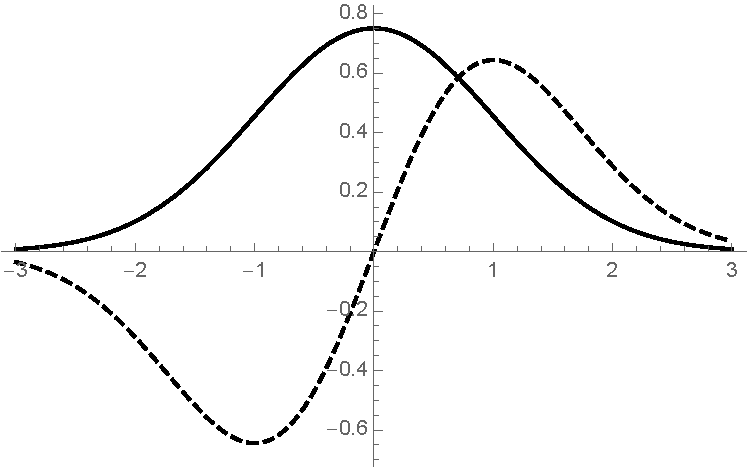
\includegraphics[width=0.5\columnwidth]{Pictures/Psi0Psi1.pdf} 
\end{center}
\caption{Fonctions d'onde des deux premiers états propres de l'oscillateur harmonique $\psi_0(x)=\langle x \vert 0\rangle$ et $\psi_1(x)=\langle x \vert 1\rangle$. }
\label{fig:Psi01}
\end{figure}

Soit l'état quantique 
\begin{equation}
\vert \psi \rangle = 
 \frac{1}{\sqrt{2}}\ket{0}  +  \frac{1}{\sqrt{2}}\ket{1}\ .
 \label{Eq:psi}
\end{equation}

\begin{enumerate}


\item 
Supposons qu'à l'instant $t=0$, l'oscillateur harmonique est dans l'état $\ket{\psi}$ donné par l'équation \eqref{Eq:psi}. Quel est son état $\ket{\psi(t)}$ à l'instant $t>0$ ?

\item 
Que vallent 
\begin{eqnarray}
&\langle P(t) \rangle = \braket{\psi (t)|\hat P|\psi(t)}&\\
&\langle X(t) \rangle = \braket{\psi(t)|\hat X|\psi(t)}&\\
&\braket{\psi(t)| \hat X^2 |\psi(t)}\quad  ?&
\end{eqnarray}




\item Soit les instants suivants 
\begin{equation}
t_k= k \frac{\pi}{4} \frac{1}{\omega}\quad , \quad k=0,1,2,3,4,5,6,7 \ .\label{Eq:tk}
\end{equation}


Les panneaux de la figure \ref{FigPsi2} représentent la densité de probabilité 
\begin{equation}
\vert \psi(x,t)\vert^2 = \vert \langle x \vert \psi(t) \rangle \vert^2
\end{equation}
 à certains instants $t$, avec $t \in \{t_0,...,t_7\}$.

De quels instants $t_k$ s'agit-il?   Justifiez votre réponse. 
(La réponse attendue est de la form "Le panneau (A) représente   $ \vert \psi(x,t)\vert^2$ aux instants $t_2$ et $t_7$ parceque... ."


\begin{figure}
    \centering
    \begin{subfigure}[t]{0.4\textwidth}
        \centering
        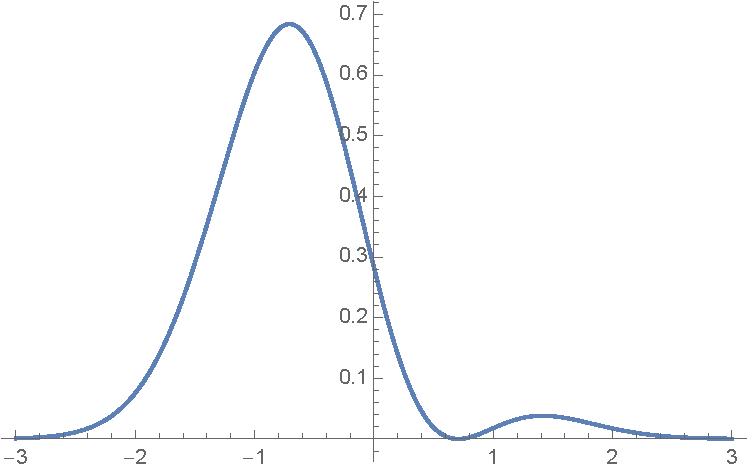
\includegraphics[width=\linewidth]{Pictures/FigPsi4.pdf}
        \caption{} \label{fig:timingA}
    \end{subfigure}
    \hfill
    \begin{subfigure}[t]{0.4\textwidth}
        \centering
        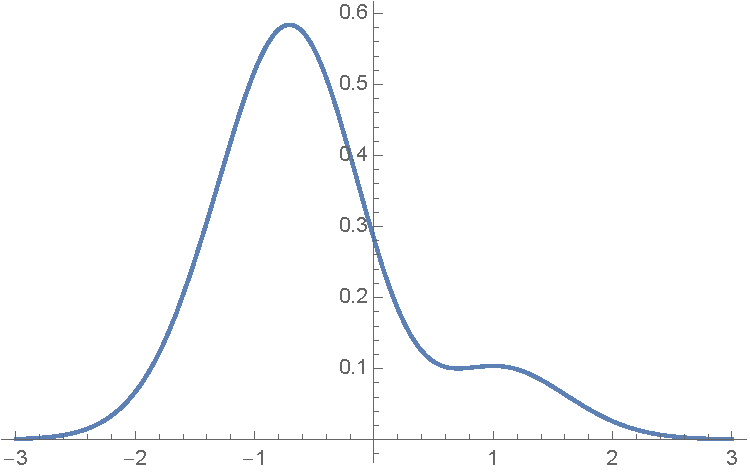
\includegraphics[width=\linewidth]{Pictures/FigPsi3.pdf} 
        \caption{} 
        \label{fig:timingB}
    \end{subfigure}
  

    \vspace{1cm}
   \begin{subfigure}[t]{0.4\textwidth}   
        \centering
        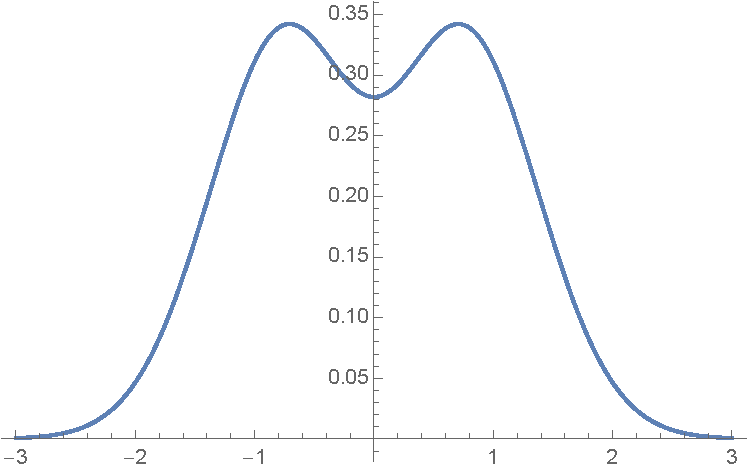
\includegraphics[width=\linewidth]{Pictures/FigPsi2.pdf}
        \caption{} \label{fig:timingC}
    \end{subfigure}
    \hfill
    \begin{subfigure}[t]{0.4\textwidth}
        \centering
        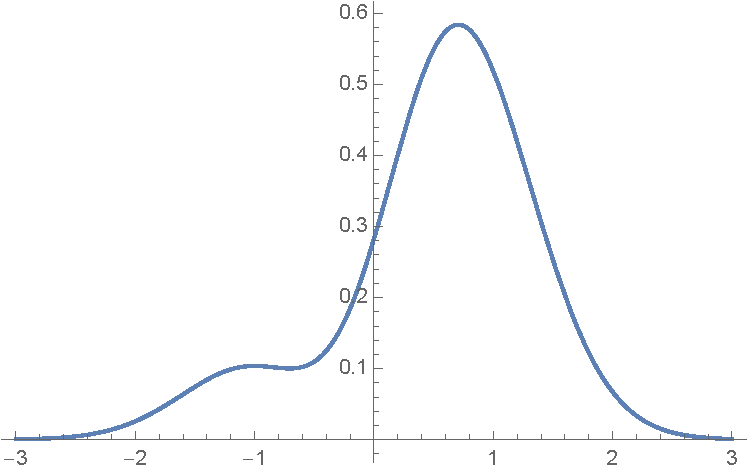
\includegraphics[width=\linewidth]{Pictures/FigPsi1.pdf} 
        \caption{} 
        \label{fig:timingD}
    \end{subfigure}
    
    \vspace{1cm}
   \begin{subfigure}[t]{0.4\textwidth}
    \hfill       
        \centering
        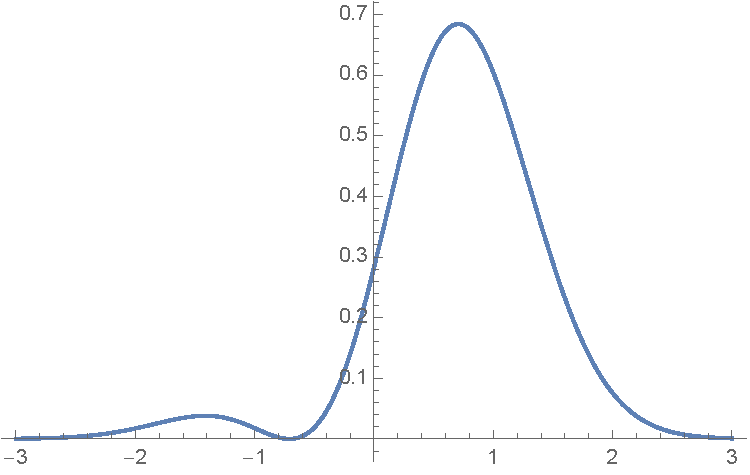
\includegraphics[width=\linewidth]{Pictures/FigPsi0.pdf}
        \caption{} \label{fig:timingE}
    \end{subfigure}
 
        
    \caption{Les panneaux (A) (B) (C) (D) (E) représentent la densité de probabilité 
$ \vert \psi(x,t)\vert^2$ à certains des instants $t_k$ donnés à l'équation \eqref{Eq:tk}.}
\label{FigPsi2}
\end{figure}





\end{enumerate}

\paragraph{Question 2} \textit{Changement de base.} \\

Les opérateurs sans dimension position $\hat x$ et impulsion $\hat p$ satisfont 
\begin{equation}
[\hat x, \hat p ] = i\ .
\label{xp:1}
\end{equation}
Les états propres de l'opérateur position sont notés $\vert x \rangle$ et satisfont
\begin{eqnarray}
\hat x \vert x \rangle &=& x\vert x \rangle \ ,\label{xp:2B}\\
\langle x' \vert x \rangle &=& \delta (x-x') \ .
\label{xp:2}
\end{eqnarray}
Pour tout état $\vert \psi \rangle$ nous avons
\begin{eqnarray}
\langle x \vert \hat x \vert \psi \rangle &=& x  \langle x  \vert \psi \rangle \ ,
\label{xp:3}\\
\langle x \vert \hat p \vert \psi \rangle &=& -i \partial_x  \langle x  \vert \psi\rangle\ . \label{xp:4}
\end{eqnarray}

Considérons les opérateurs obtenus par une rotation d'angle $\theta$ de l'espace des phases
\begin{eqnarray}
\hat u  &=&  \cos \theta\  \hat x + \sin \theta\   \hat p\ ,
\label{xp:5}\\
\hat v  &=&  - \sin \theta \  \hat x + \cos \theta \  \hat p \label{xp:6}\ .
\end{eqnarray}
Nous avons aussi la transformation inverse
\begin{eqnarray}
\hat x  &=&  \cos \theta\   \hat u - \sin \theta\   \hat v\ ,
\label{xp:7}\\
\hat p  &=&   \sin \theta\   \hat u + \cos \theta\   \hat v \label{xp:8}\ .
\end{eqnarray}
Ces opérateurs satisfont 
\begin{equation}
[\hat u, \hat v ] = i\ .
\label{xp:9}
\end{equation}
Soit $\vert u \rangle$ les états propres de $\hat u$:
\begin{equation}
\hat u \vert u \rangle = u \vert u \rangle \ .
\label{xp:10}
\end{equation}
Pour tout état $\vert \psi \rangle$ nous avons par conséquent, par analogie avec \eqref{xp:2B} et \eqref{xp:2} 
\begin{eqnarray}
\langle u \vert \hat u \vert \psi \rangle &=& u  \langle u  \vert \psi \rangle \ ,
\label{xp:3}\\
\langle u \vert \hat v \vert \psi \rangle &=& -i \partial_u  \langle u  \vert \psi \rangle\ . \label{xp:4}
\end{eqnarray}

Le but de cette qustion est d'établir la forme du changement de base $\langle x \vert u \rangle$.

\begin{enumerate}


\item 
Démontrer  à partir de la définition de $\hat u$ et $\hat v$ donnée dans  \eqref{xp:5} et \eqref{xp:6} la relation de commutation  $[\hat u, \hat v ] = i$.

\item
Considérer les grandeurs $\langle x \vert \hat u \vert u\rangle $ et $\langle x \vert \hat x \vert u\rangle$. En utilisant les relations données ci-dessus, réexprimer ces grandeurs comme deux équations différentielles pour $\langle x \vert u\rangle$, l'une impliquant une dérivée par rapport à $u$ et l'autre une dérivée par rapport à $x$.

\item
Résoudre ces équations différentielles, et montrer que leur solution est
\begin{equation}
\langle x \vert u \rangle =  c  \exp \left( - i \frac{\cos \theta}{\sin \theta}\frac{x^2}{2} + i \frac{u x}{\sin \theta} - i \frac{\cos \theta}{\sin \theta}\frac{u^2}{2} \right)
\end{equation}
avec $c$ une constante.

\item
Déterminer la valeur de $c$ pour que 
\begin{equation}
\langle u' \vert u \rangle = \int dx \langle u' \vert x \rangle \langle x \vert u \rangle = \delta (u - u') \ .
\end{equation}
\end{enumerate}

\paragraph{Question 3} \textit{Interférometre de Mach-Zehnder avec pertes dans un bras.} \\

\begin{figure}[h!]
\begin{center}
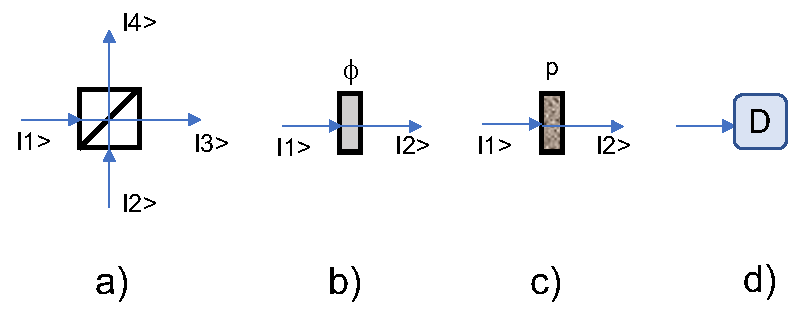
\includegraphics[scale=0.9]{Pictures/Fig-Optique.pdf} 
\end{center}
\caption{Elements optiques: a) séparateur de faisceau 50/50; b) lame de phase; c) lame absorbante ; d) détecteur.}
\label{fig:Optique}
\end{figure}

La figure \ref{fig:Optique} réprésente 4 éléments optiques.

Le panneau a) représente un séparateur de faisceau 50/50. Les ports d'entrée et de sortie sont notés 1,2 et 3,4 respectivement. Si un photon entre par le port 1, ou par le le port 2, il subit la transformation
\begin{eqnarray}
\vert 1 \rangle &\to & \frac{1}{\sqrt{2}} \vert 3 \rangle + \frac{i}{\sqrt{2}} \vert 4 \rangle \\
\vert 2 \rangle &\to & \frac{i}{\sqrt{2}} \vert 3 \rangle + \frac{1}{\sqrt{2}} \vert 4 \rangle 
\end{eqnarray}
(noter les facteur $i$ qui rendent cette transformation unitaire).

Le panneau b) représente une lame de phase qui réalise la transformation
\begin{eqnarray}
\vert 1 \rangle &\to & e^{i \phi}  \vert 2 \rangle \ .
\label{Eq:opt3}
\end{eqnarray}

Le panneau c) représente une lame absorbante. Cette lame absorbe le photon avec une probabilité $p$ et laisse passer le photon avec une probabilité $1-p$. Nous pouvons modéliser la lame absorbante par la transformation
\begin{eqnarray}
\vert 1 \rangle &\to & \sqrt{p}  \vert ABS \rangle + \sqrt{1-p}  \vert 2 \rangle 
\end{eqnarray}
ou $\vert ABS \rangle$ représente l'état si le photon est absorbé, et $\vert 2 \rangle $ représente le photon si il a traversé la lame sans être absorbé.

d) représente un détecteur de photon unique.



\begin{figure}[h!]
\begin{center}
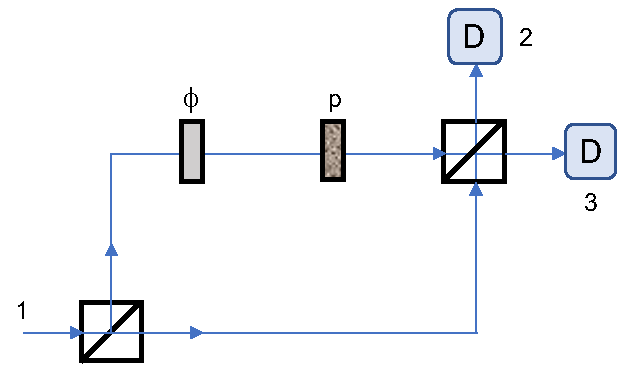
\includegraphics[width=0.5\columnwidth]{Pictures/Fig-Interf.pdf} 
\end{center}
\caption{Interférometre de Mach-Zehnder dans un bras duquel on a mis une lame de phase et une lame absorbante.}
\label{fig:MZ}
\end{figure}


La figure \ref{fig:MZ} représente un interférometre de Mach-Zehnder dans un bras duquel on a mis une lame de phase et une lame absorbante.  Le port d'entrée du photon est noté $1$, et les deux ports de sortie $2$ et $3$.

\begin{enumerate}
\item Expliquer pourquoi, si la probabilité que la lame absorbante absorbe le photon est $p$, l'équation \eqref{Eq:opt3} qui permet de décrire son action sur un photon contiens des facteurs $\sqrt{p}$ et $\sqrt{1-p}$. Pourquoi ces racines carrées?

\item 
Supposons qu'un photon entre par le port $1$ de l'interférometre de la figure \ref{fig:MZ}. L'état final du photon peut s'écrire comme une combinaison linéaire des états $ \vert ABS \rangle $, $ \vert 2 \rangle $ et $ \vert 3 \rangle $. Donner cet état final en fonction de $\phi$ et $p$.

\item Donner la probabilité de trouver le photon dans les ports $2$ et $3$ de l'interférometre en  fonction de $\phi$ et $p$.

\item Pour $p$ donné, quel est la valeur minimale de trouver le photon dans le port $2$ (lorsqu'on varie $\phi$).

\item Représenter dans un graphique la probabilité de trouver le photon dans le port 2 en fonction de $\phi$, lorsque $p=1/3$. (Utiliser la page quadrillée).


\end{enumerate}

%\begin{center}
%\begin{tikzpicture}
%\def\sizx{15};
%\def\sizy{22};
%\draw[help lines, step = 0.5cm] (0,0) grid (\sizx, \sizy);
%\end{tikzpicture}
%\end{center}